\documentclass[11pt]{article}
\usepackage[T1]{fontenc}
\usepackage{lmodern,amsmath,amssymb,booktabs,graphicx}
\usepackage[letterpaper,left=0.86in,right=0.86in,top=0.82in,bottom=0.84in]{geometry}
\usepackage[hidelinks,pdfauthor={qiyuanhuakai},pdftitle={Photon-number calibration of a dual-readout Gaussian boson sampler}]{hyperref}
\newcommand{\OpticalNull}{24.46\% (23.60--25.53\%)}
\newcommand{\TiltNull}{24.56\% (23.50--25.73\%)}
\newcommand{\PairNull}{0.96\% (0.44--1.76\%)}

\newcommand{\BenchRows}{%
Direct clicks (GPU) & 0.131 & 0.154 & 25.934 & --- \\%
PNR (GPU) & 0.077 & 0.080 & 24.247 & 1.051 \\%
PE--PNR (CPU) & 27,875.571 & 437,468.584 & 24.229 & 1.325 \\%
PE--PNR (GPU) & 15,145.428 & 575,287.109 & 24.217 & 0.916 \\%
Frugal $K=2$ (CPU) & 9.985 & 10.399 & 55.688 & --- \\%
Frugal $K=4$ (CPU) & 27.286 & 27.239 & 37.425 & --- \\%
}

\newcommand{\TV}{d_{\mathrm{TV}}}
\newcommand{\tr}{\operatorname{Tr}}
\newcommand{\E}{\mathbb{E}}
\newcommand{\resource}{\href{https://github.com/qiyuanhuakai/deziroGBS/tree/archive/iteration115-visible-sectors-v3}{archived implementation and data}}
\setlength{\parskip}{1.5pt}
\setlength{\emergencystretch}{2em}
\title{\bfseries Photon-number calibration of a dual-readout\\ Gaussian boson sampler}
\author{qiyuanhuakai}
\date{27 November 2026}
\begin{document}
\maketitle
\begin{abstract}
A fast optical surrogate may reproduce the number of photons in a shot while misplacing them across output channels. We use a positive mixture of number-filtered Gaussian states to calibrate the total count of a lossy Gaussian boson sampler. The mixture gives both photon-number-resolving (PNR) and direct threshold samples and preserves the base model's conditional distribution within each photon-number sector. On a two-spectrum model of the high-power Jiuzhang~3.0 circuit with 1,152 multiplexed outputs, seven components fitted directly to the optical total-count law reduce its numerical total variation (TV) upper bound from $2.74083\%$ to $0.000838\%$. Batched PNR and direct-click throughput is $0.346$ and $1.056\,\mu$s per full record, respectively. On a selected pair of eight-detector banks, a separate calculation bounds the full 16-channel PNR error between $2.1671\%$ and $3.1080\%$ and gives a full click-pattern error of $2.1221\%$. On the same panel, an independent adaptation of the corrected positive-$P$ sampler gives $0.336\%$ click TV. A correlated bright-mode projection gives $0.0311\%$ and reduces the error in a spatial vacuum probability at fixed whole-device photon number. The batched throughput belongs to the original number-tilted sampler.
\end{abstract}

\section{Introduction}
A multiplexed optical experiment reports which detectors fired. Numerical models can also return the number of photons at each detector before thresholding. The two tasks probe distinct approximations. A simulator can cheaply draw an accurate total photon number from a Gaussian generating function \cite{avagyan} and still assign photons incorrectly across detectors. Conversely, a model of a binary output such as FrugalGBS \cite{frugal} can be tested on complete click probabilities, but its samples alone do not specify the underlying multiplicities.

We study whether a fast spatial model can acquire an accurate total count without giving up either readout. The experiment is motivated by the high-power configuration of Jiuzhang~3.0 \cite{jiuzhang}. Its calibrated optical transfer and two squeezing spectra specify a target; separately recorded clicks provide a hardware comparison. Gaussian decomposition into classical displacement and a quantum residual underlies previous simulations of lossy GBS \cite{oh}. The number filter $g^{\hat N}$ also has a well-developed Gaussian theory \cite{walk}. Here we combine a spatially local residual with a positive mixture of these filters, fit the mixture solely to optical total counts, and quantify what this operation changes in both readouts. Low-order marginal matching has been used to build GBS surrogates \cite{villalonga}; grouped phase-space observables can test experiments without drawing detector records \cite{dellios}. Goodman et al.\ subsequently give explicit output sampling rules for both detectors \cite{goodman}. We evaluate an independent adaptation against the same optical panel. A second contribution is an independently computable bracket on the full PNR distribution of two multiplexed banks. It makes the remaining spatial bias visible at the same input and resolution used for the speed comparison.

\section{Optical model and positive number calibration}
Let $T$ be the lossy transfer on the measured channels, and let $V$ denote a quadrature covariance in units of vacuum variance one. For one centered spectrum write $X=(V-I)/2$. For the two independent spectra, the total photon number $N$ has generating function
\begin{equation}
 G_P(z)=\prod_{s=1}^{2}\det[I+(1-z)X_s]^{-1/2}.
 \label{eq:pgf}
\end{equation}
The square root is continued from $z=1$. For eigenvalues $e_i$ over both spectra, $p_0=\prod_i(1+e_i)^{-1/2}$ and
$2n p_n=\sum_{j=1}^{n}p_{n-j}\sum_i[e_i/(1+e_i)]^j$.
We evaluated this recurrence at 65 decimal digits with double-precision covariance eigenvalues. The optical mean is 116.286 detected photons at the original power.

\paragraph{Base state.}
We complete each transfer with environment modes $E=(I-T^\dagger T)^{1/2}$ and condition on a commuting set of environment momentum quadratures. Gaussian conditioning gives a covariance $V_c=V_{vv}-V_{ve}V_{ee}^{-1}V_{ev}$ and a mean linear in a real standard Gaussian latent vector. On the full visible circuit the two residuals are pure to a numerical symplectic check and carry mean photon numbers 3.546 and 0.820. Correlated classical displacements account for the remaining 111.92 mean photons. For the fast base model we first compress each eight-channel bank to the leading left singular direction of its $8\times 50$ transfer. The squared moduli of that direction determine eight unequal splitter fractions. We condition the compressed transfer as above, retain the common random displacements, and replace the residual state by the product of its single-bank Gaussian marginals. This last step removes part of the cross-bank interference. The base is a normalized physical state, with a total-count generating function $G_Q$.

\paragraph{Positive mixture.}
Given the base state $\rho$, admissible $z>0$ satisfy $G_Q(z)<\infty$. Define
\begin{equation}
 \rho_z=\frac{z^{\hat N/2}\rho\,z^{\hat N/2}}{G_Q(z)},\qquad
 \rho_*=\sum_{k=1}^{K}w_k\rho_{z_k},\quad w_k\ge0,\quad\sum_k w_k=1 .
 \label{eq:filter}
\end{equation}
This filter is used computationally. Evaluation requires one mixture draw per record. Let $q(x)$ denote the base PNR probability and $n=|x|$. Then
\begin{equation}
 q_*(x)=q(x)r_n,\qquad r_n=\sum_k w_k z_k^n/G_Q(z_k).
 \label{eq:sectors}
\end{equation}
This identity also holds when the spectra are unresolved because their combined total is fixed at $n$.

\paragraph{What calibration can establish.}
Equation~\eqref{eq:sectors} proves $Q_*(x\mid N)=Q(x\mid N)$ wherever the conditional is defined. Summing the absolute probability change within each sector gives $\TV(Q_*,Q)=\TV(Q_{*,N},Q_N)$ for the full PNR measurement. For a target $P$ supported on the base support, the chain rule yields
\begin{equation}
 D(P\Vert Q_*)=D(P_N\Vert Q_{*,N})+
      \E_{P_N}D\big(P(\cdot\mid N)\Vert Q(\cdot\mid N)\big).
 \label{eq:kl}
\end{equation}
Thus any decrease in total-count relative entropy carries exactly to full PNR relative entropy, whenever the terms are finite. A decrease in total-count TV alone has no such implication for TV to $P$. Even attainable total-count corrections are restricted: $r_n^2\le r_{n-1}r_{n+1}$ by Cauchy--Schwarz applied to the positive exponential mixture. These properties explain both the strong correction in the total count and its failure to remove conditional spatial error.

\section{Fitting and sampling both readouts}
\paragraph{Fit.}
For the benchmark sampler we use a uniform grid of 25 log gains on $[-0.1,0.1]$ and remove points beyond the convergence boundary. In bins $0\le n\le440$ we use nonnegative least squares on columns $q_n z_k^n/G_Q(z_k)$ against the optical $p_n$, discard weights below $10^{-10}$, and renormalize. Seven weights remain. The retained log gains range from $-0.10$ to $0.01667$; their full-precision values and weights are archived. Neither hardware capture enters the fit.

\paragraph{Gaussian realization.}
Use real coordinates for the complex coherent amplitudes and rotate each conditional covariance block into its eigenbasis. Write the row of field coordinates as $u^\mathsf{T}A$, with $u$ standard normal, and denote the conditional eigenvalues of $X$ by $e_i$. For a given $z$ put $d_i=1+(1-z)e_i$. Multiplying the conditional generating function by the number filter and completing the square gives
\begin{align}
 e_i'&=ze_i/d_i, & A'&= A\,\mathrm{diag}(\sqrt{z}/d_i),\\
 \mathrm{Cov}(u\mid z)^{-1}
     &=I+2(1-z)A\,\mathrm{diag}(d_i^{-1})A^\mathsf T. \label{eq:latent}
\end{align}
For example, each real coordinate contributes a factor
$d_i^{-1/2}\exp[-(1-z)a_i^2/d_i]$ to the normalizer at field $a_i$. Integrating these factors over $u$ gives Eq.~\eqref{eq:latent}. Its log normalizer agrees with the unrestricted eigenvalue calculation to $1.8\times10^{-15}$ on the seven components. Both spectra share a mixture label drawn once for the entire shot. Conditional on that label the spectral fields are independent.

\paragraph{Readout.}
After drawing the transformed latent field, all banks can be sampled in parallel. For each spectrum and bank, the generating function at $1-w$ is
\begin{equation}
 \prod_{i=1}^2(1+w e'_i)^{-1/2}
       \exp\!\left[-\sum_{i=1}^2 w(a'_i)^2/(1+w e'_i)\right].
 \label{eq:bank}
\end{equation}
The PNR path draws a bank count from the coefficients of the two-spectrum product, then distributes the photons multinomially using the eight splitter fractions. The direct-click path evaluates Eq.~\eqref{eq:bank} with $w$ equal to the sum of fractions in a subset of detectors. These are subset-vacuum probabilities; inclusion--exclusion gives the 256 click-pattern probabilities \cite{threshold}. This path draws a binary outcome directly. For $B$ banks, latent dimension $d$, and fixed bank width, dense field preparation per shot costs $O(d^2+Bd)$ plus readout and output. Direct readout enumerates subsets within a bank; PNR recurrence cost depends on the drawn number. Scaling in bank width or excited-input rank can therefore change the throughput substantially.

\section{Full-circuit total counts and spatial tests}
We use $\TV(p,q)=\frac12\sum_i|p_i-q_i|$. To bound a total-count TV after cutoff $L$, we add half the sum of the two tail masses to half the absolute discrepancy in bins $0,\ldots,L$. The original-power seven-component mixture gives $8.3787\times10^{-6}$, compared with $2.7408325\times10^{-2}$ before calibration. Optical and mixture mass beyond $L=440$ is approximately $5.02\times10^{-11}$ and $4.89\times10^{-15}$, respectively. These are numerical model-to-model results. The maximum empirical CDF discrepancy from 131,072 PNR draws is $0.00248$.

\begin{figure}[ht]
\centering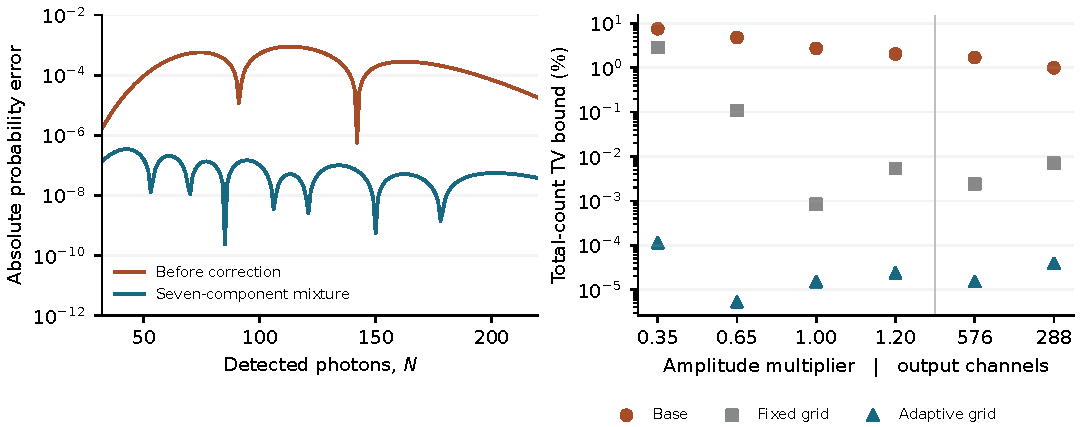
\includegraphics[width=.96\linewidth]{total-counts.pdf}
\caption{Left: absolute errors in individual photon-count probabilities for the original seven-component sampler. Right: refits trained only on even counts, evaluated using all counts. The first four settings rescale $\sinh r$ at 1,152 outputs; the last two retain the first 576 or 288 output channels at original gain.}
\label{fig:total}
\end{figure}

For a stress test we independently refit each of six settings on even counts through 480. An expanded grid augments the original candidates with 49 log gains from $-12h$ to $6h$, where $h=\sqrt{\max(0,v_P-v_Q)}/v_Q$ and $v_P,v_Q$ are variances on the normalized even training bins. Odd counts and all spatial observations are held out. Across means of 14.25 to 167.45 photons, the adaptive fits give all-bin TV upper estimates of $5.28\times10^{-8}$ to $1.14\times10^{-6}$ and conditional odd-bin TV of $5.27\times10^{-8}$ to $2.24\times10^{-6}$. We additionally evaluated the prepared component covariances at 28 complex generating-function arguments; the largest discrepancy with the stored coefficients was $7.55\times10^{-10}$. This is an interpolation test of probability bins on related circuits. The reported GPU speed belongs to the original seven-component model.

On a single bank, calibration increases mean eight-bit TV from $0.00667\%$ to $0.07106\%$ against full optical probabilities. For all $\binom{144}{2}=10,296$ bank pairs we compared the joint distribution of two click multiplicities (81 outcomes). Average TV to hardware files 10 and 11 is $1.3437\%$ and $1.3302\%$; the corresponding file-to-file distance is $0.1793\%$. The captures contain 1,601,553 and 1,584,835 high-power shots. Their photon multiplicities within a fired detector are unobserved. Full-width direct-click total histograms have empirical TV $4.1069\%$ and $4.0163\%$ to these files; thresholding independently generated PNR rows gives $4.3625\%$ and $4.2675\%$.

\begin{figure}[ht]
\centering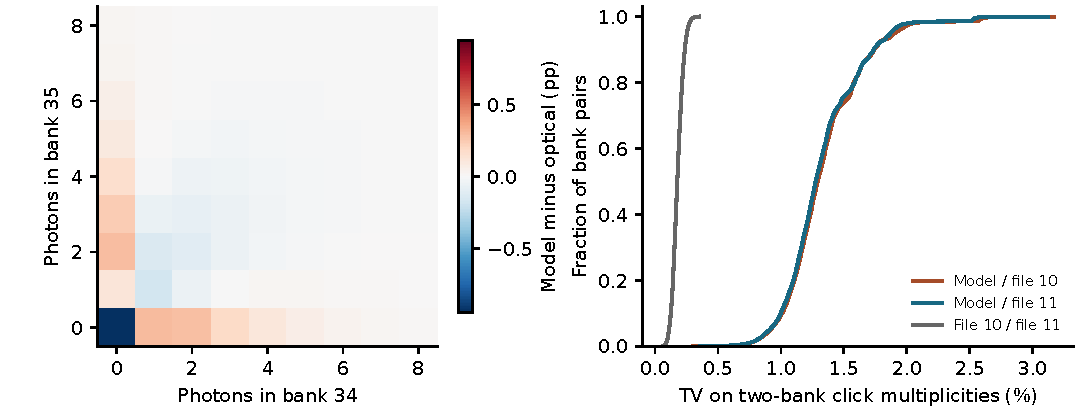
\includegraphics[width=.95\linewidth]{spatial-errors.pdf}
\caption{Left: signed error in joint \emph{photon} totals of banks 34 and 35 (percentage points per cell; counts up to eight displayed). Right: empirical distribution across all spatial pairs of the TV in two \emph{click} multiplicities. The two public captures are independent files from the same experimental configuration.}
\label{fig:spatial}
\end{figure}

\section{A matched 4,096-shot comparison}
We retain channels 272--287 (zero-based), the eight channels of each of banks 34 and 35, with all other channels traced out. This panel had a large spatial residual in our earlier diagnostic; it is a diagnostic stress case selected with knowledge of the optical discrepancy. Every method uses the same two-spectrum reduced optical input or the corresponding marginal of the calibrated surrogate. Optical threshold probabilities for all $2^{16}$ words are enumerated by high-precision subset-vacuum inversion. The two-channel PNR diagnostic uses channels 272 and 280, one per bank, and saturates each count at eight. Its 81 reference probabilities use the bivariate Gaussian determinant recurrence with overflow probabilities recovered from the one-dimensional marginals.

\begin{table}[ht]
\centering
\caption{Single-machine measurements on the same 16-channel panel. Time is in $\mu$s per record; empirical TVs are percentages against the optical reference. PE denotes the upstream \texttt{photonic-engines} PNR implementation. PNR rows are also thresholded for the click column.}
\small
\begin{tabular}{lrrrr}
\toprule
& \multicolumn{2}{c}{Time per record} & \multicolumn{2}{c}{Empirical TV (\%)}\\
\cmidrule(lr){2-3}\cmidrule(lr){4-5}
Sampler & Median & Mean & 16-bit clicks & Two-channel PNR\\
\midrule
\BenchRows
\bottomrule
\end{tabular}
\label{tab:matched}
\end{table}

For the approximation, the full click-word TV from the two calculated laws is $2.12210\%$; our two-channel capped-PNR model TV is $0.22298\%$. On full click words the Frugal $K=2$ and $K=4$ model TVs are $47.5135\%$ and $21.7250\%$, respectively, obtained by summing both complete conditional trees and combining the spectra. These quantities measure model bias. An empirical histogram of 4,096 words is sparse across 65,536 cells. In 1,000 independent multinomial simulations the plug-in TV of optical draws against optical truth had median \OpticalNull; for mixture draws against optical truth it was \TiltNull. Parentheses give the central 95\% simulation ranges. For the 81-cell PNR observable the optical null gave \PairNull. The scored direct-click TV of 25.93\% falls above the 97.5th percentile of the mixture simulation. In a post hoc replication of 64 fresh 4,096-shot GPU batches the median was 24.42\%, and 3 batches reached or exceeded 25.93\%. The original scored batch remains in Table~\ref{tab:matched}. These quantiles characterize sampling variability for this statistic, rather than uncertainty in the analytic model TV.

\paragraph{Sampling protocol.}
The tilted GPU kernel used 10 batches of 4,096, discarding the first for timing and scoring the final batch. Frugal used six such batches per cutoff with five timed; the final batch was scored. PE sampled the reduced state via a 32-mode Gaussian purification per spectrum, discarded the purifying modes and added the two spectra. Covariance reconstruction error was at most $5.25\times10^{-13}$. Each PE device used 32 blocks of 128, excluding the first block for timing and scoring all 4,096 outcomes. The archived run checks every block for censoring at the 100-photon budget. The PE CPU and CUDA configurations use distinct seeds; the two spectra and the 32 blocks have distinct seed domains within each backend. The mean over the equal-sized timed blocks includes rare expensive trajectories. Table~\ref{tab:matched} compares the indicated operating points. At 16 channels, the original optical law took 2.93 s to enumerate. The exact categorical cache subsequently took $0.0229\,\mu$s per row with $2^{16}$ stored probabilities, faster than either online readout here. Its table grows exponentially in channel count. In the PNR samples, the joint bank-total histogram had 4.398\% empirical TV against optics; the central 95\% optical-null range was 3.105--4.775\%.

\section{Bounding the full 16-channel PNR distribution}
A two-detector marginal alone cannot establish the quality of a full PNR vector. For this panel we can bracket the TV numerically without enumerating the infinite 16-dimensional Fock basis. Let $P$ be the optical law, $Q_*$ the surrogate, and let $C=(N_A,N_B)$ record the total photons in each bank. On a $128^2$ torus we evaluate the two-variable characteristic function
\begin{equation}
 \E[z^{N_A}w^{N_B}]
 =\prod_s\det(I+X_s)^{-1/2}
       \det(I-ZK_s)^{-1/2},\qquad
 K_s=I-(I+X_s)^{-1},
 \label{eq:torus}
\end{equation}
where $Z$ repeats the bank fugacities on both quadratures. Factor the second determinant by its $A$ block: the $B$ factor uses $K_{BB}+zK_{BA}(I-zK_{AA})^{-1}K_{AB}$. We sum principal logarithms of the individual factors continued from the vacuum generating function. A discrete Fourier transform yields the nonnegative law of the bank totals modulo 128 up to rounding. Folding onto $64^2$ agrees with a separate evaluation to $10^{-14}$. Coarse graining gives $\TV(P,Q_*)\geq\TV(P_{C\bmod128},Q_{*,C\bmod128})=2.16708\%$.

For an upper bound, rotate each target bank to its bright singular direction and project the other seven directions onto vacuum. Write $P_b$ for the normalized projected-state law and $\epsilon$ for the original probability of at least one dark photon. A projection of a purification gives trace distance at most $\sqrt\epsilon$ after normalization and partial trace. The conditional covariance of the two bright modes follows from the vacuum Schur complement. Both $P_b$ and $Q_*$ now have the same downstream splitting for a given bank total: independent multinomial splitting within banks, with the same detector fractions in both spectra. Disjoint supports for different totals imply
$\TV(P_b,Q_*)=\TV((P_b)_C,(Q_*)_C)$. Modulo aliasing changes this comparison by at most the sum of the two photon tails above 127 (each below $10^{-16}$ numerically). We find
\begin{equation}
 \epsilon=8.8322\times10^{-5},\quad
 \TV((P_b)_{C\bmod128},(Q_*)_{C\bmod128})=2.16820\%,
 \quad \TV(P,Q_*)\ \le\ 3.1080\% .
\end{equation}
As a further check, we split the model bank-count law onto the detectors, aggregate to 81 click multiplicities, and compare to an independent enumeration of all 65,536 threshold words. The largest single-cell probability discrepancy is $1.16\times10^{-12}$. The bounds pertain to the mathematical readout model and the supplied covariance; floating-point evaluations are not interval-certified. The panel lower bound also applies to the full circuit by marginalization. The panel upper bound does not. For all 1,152 channels a numerical Gaussian-fidelity calculation \cite{fidelity} gives only a $99.633\%$ upper estimate. The gap between these constraints remains large.

\section{Comparison with corrected positive-\texorpdfstring{$P$}{P} sampling}
Goodman et al.~\cite{goodman} report a phase-space sampler tested up to 1,152 outputs. Their Jiuzhang~3 comparisons include grouped click counts and marginals through order 20 and use one million shots. They distinguish the original optical parameters from a target with a refitted transmission and decoherence. Their article describes separate prescriptions for threshold and PNR detectors. We compare the original-power optical target on banks 34 and 35, using no hardware-fitted parameters. A panel-specific fit can differ from the marginal of a fit on all 1,152 outputs.

We independently implemented their Eqs.~(8)--(12) for this panel. The two spectra supply independent positive-$P$ trajectories. We sum their complex intensities before applying the threshold vacuum-probability or PNR intensity projection. For each readout, 131,072 training trajectories determine ten successive whitening, coloring and clipping maps. We use analytic target means and covariances (including the repeated-index second moments) and hold the maps fixed for evaluation. Both target covariance matrices were positive definite. The numerical implementation and timings are ours. The authors identify XQSIM as their MATLAB package and offer the paper's sampler data on request; our experiment uses their published equations and the deziroGBS input.

\begin{table}[ht]
\centering\small
\caption{Bank pair 34,35 at original power. Click errors use all 65,536 words. The PNR comparison in the last column uses the same two capped channels for all rows with an entry. Intervals for the positive-$P$ rows have simultaneous 99\% coverage conditional on the trained maps.}
\begin{tabular}{lrr}
\toprule
Model and readout & Full click TV (\%) & Two-channel PNR TV (\%)\\
\midrule
Number-tilted sampler & 2.1221 & 0.2230\\
Positive-$P$, direct clicks & 0.3358 \quad [0.0806, 0.5105] & ---\\
Positive-$P$, PNR then threshold & 0.3398 \quad [0.0952, 0.5145] & 0.0164 \quad [0, 0.1911]\\
Correlated bright-mode projection & 0.03114 & ---\\
\bottomrule
\end{tabular}
\label{tab:positivep}
\end{table}

For the positive-$P$ rows we integrate the conditional output probabilities over $m=1,048,576$ fresh trajectories per readout. Each trajectory supplies a normalized 65,536-entry probability vector, factored into two 256-word tables. For the PNR diagnostic it supplies a product of two capped Poisson laws. For a reference $p$ and mean estimate $\hat q$, convexity gives $\TV(q,p)\le\E\TV(\hat q,p)$. Replacing one trajectory changes this statistic by at most $1/m$. Bounded differences therefore give the upper endpoint $\TV(\hat q,p)+\sqrt{\log(1/\alpha)/(2m)}$. For the lower endpoint the first half selects the set where its estimate exceeds $p$; the second half estimates that event's excess probability with a one-sided Hoeffding bound. We allocate $\alpha=0.01/6$ to each tail across three comparisons. The intervals account for finite integration error with fixed training, not optical calibration uncertainty. The corrected positive-$P$ readout is more accurate than the fast tilted sampler on this stress panel by either matched diagnostic. In a separate run of 524,288 output draws per route, the independent four-thread CPU/BLAS implementation took 4.77 and 4.65~$\mu$s per row for direct clicks and PNR (batch 8,192; field generation through sampled output). These cannot establish a hardware-matched speed ranking against the original MATLAB implementation.

\section{Spatial error at fixed whole-device photon number}
To test which approximation matters spatially, we constructed a second physical state from the same optical transfer. In each bank, retain the first $k$ left singular directions of its transfer. Condition all discarded directions across the entire circuit on vacuum, keep the full Gaussian correlations on the retained directions, and embed the state back through the original bank splitters. This calculation uses the optical transfer alone and does not fit any total-count or spatial probabilities. If $\epsilon$ is the probability that at least one discarded mode contains a photon, projecting a purification gives
\begin{equation}
 \TV(P_{\rm meas},Q^{(k)}_{\rm meas})\leq\sqrt{\epsilon},
 \qquad 1-\epsilon=\prod_s\det(I+X_{s,\mathrm{dark}})^{-1/2}.
\end{equation}
The inequality holds before the choice of PNR or threshold measurement. For $k=1,2,4$, the numerical whole-circuit ceilings are respectively $7.918\%$, $6.741\%$ and $4.922\%$, retaining 144, 288 and 576 optical directions per spectrum. These are projection guarantees for a correlated Gaussian state. End-to-end sampling of its full correlated brightness pattern was not timed. The original fast factorized sampler retains its separate $99.633\%$ numerical ceiling.

With $k=1$, exact threshold enumeration on the original 34,35 panel gives $0.03114\%$ TV for the projected state, a factor of 68.1 below the tilted sampler. For five additional bank pairs (0,1), (17,89), (45,98), (71,72) and (102,143), the projected click TVs range from $0.01654\%$ to $0.02613\%$; all five decrease. These pairs cover adjacent and separated banks and do not constitute a random population sample. Applying the two-bank PNR argument above to the new state gives approximately $0.00987\%$ to $0.94753\%$ on the stress panel. Even the upper endpoint lies below the old $2.16708\%$ lower bound. All these distances are to the original optical law.

For an event that depends explicitly on the spatial distribution at \emph{fixed global} $N$, let $A$ denote no photons in the selected 16 channels. Compute $P(A\mid N=n)$ as the ratio of the $n$th coefficients of the vacuum-restricted and full generating functions. The numerator is $G(z)$ times the vacuum probability on those channels in the number-filtered Gaussian state. We evaluate the coefficients by Fourier inversion; a Chernoff bound on aliasing mass beyond 511 is below $4.2\times10^{-18}$ for the tested models. A second calculation, using a vacuum Schur complement followed by a univariate coefficient recurrence, agrees within $4.0\times10^{-15}$ on the two independently checked pairs for the target and projection. At whole-device $N=116$, the optical empty-panel probability is $30.51857\%$, the tilted model gives $29.57056\%$, and the correlated projection gives $30.51931\%$. Over $N=80,100,116,140,160$ on the stress panel the largest absolute error falls from 1.0593 to 0.000858 percentage points. This establishes improvement of a conditional spatial event and of complete panel distributions; full conditional TV on the entire device requires additional information.

\section{Throughput, limitations and reproducibility}
On an NVIDIA GeForce RTX 5080 Laptop GPU, preparing the full circuit took 1.76 s. For 16,384-record batches, median throughput including transfer of complete records to host was $0.346\,\mu$s/PNR record and $1.056\,\mu$s/direct-click record. For batches of 4,096 the corresponding values were $0.455$ and $1.162\,\mu$s. Relative to the $1.27\,\mu$s hardware record time reported for Jiuzhang~3.0 \cite{jiuzhang}, the larger batches generate 3.67 and 1.20 times as many records per second; the hardware outputs pseudo-PNR clicks, and the spatial discrepancies measured above apply. Neither the batching nor the approximation gives an exact-sampling speed claim. In 32,768 matched-randomness comparisons of FP32 and FP64 field arithmetic, zero PNR rows and 23 direct-click rows differed. These are implementation comparisons, separate from the analytic optical-model error.

Total calibration preserves useful structure: each shot is a draw from a single state shared by two measurements, and its change of probability across number sectors is exactly characterized. Its main weakness is equally specific. At fixed $N$ the surrogate has lost part of the residual interference across banks and no number filter can restore it. The correlated projection tests that explanation and improves the measured spatial errors. Computing full-device records from its retained joint state at the speed of the factorized model remains an open algorithmic task. The 128-shot pilot and this 4,096-shot run share some seeds and are reported separately. The present study covers a calibrated experimental circuit and related restrictions of it. Performance at arbitrary source rank, loss and connectivity remains outside its evidence.

\paragraph{Code, data and environment.}
The \resource{} contains the C++/CUDA sampling kernels, Python orchestration, numerical arrays, timings, verification scripts and SHA-256 checksums. The fixed tag is \texttt{archive/iteration115-visible-sectors-v3}. Official hardware archives and file digests are indexed in the repository. To reproduce the matched results, run the round-115 preparation commands in the archived checkpoint, then run
\texttt{iteration115\_panel\_v1.py} with 4,096 shots and block size 128, followed by \texttt{iteration115\_panel\_accuracy\_v2.py} in preparation and completion modes. The archived transfer file holds the calibrated matrix, detector permutation, and high-power squeezing of 25 paired sources. The supplement records its SHA-256 digest and the seed domains. Timings used an Intel Core Ultra 9 275HX, the above GPU, PyTorch 2.12.1+cu130 and CUDA 13.5 compilation. The archived adapters pin \href{https://github.com/tomdodd4598/FrugalGBS/tree/fa8b796f2afebd4845a2e335e457735952617ef8}{FrugalGBS} and \href{https://github.com/Quandela/photonic-engines/tree/6c1ed6f8f11ffc9f3c268757f0fe0bd48a768d82}{photonic-engines}. Hardware records were used for assessment only and were also examined in earlier stages of the project.

\paragraph{Use of AI tools.}
qiyuanhuakai directed the research questions, requested the dual-readout and accuracy comparisons, and raised the earlier random-stream validation issue. OpenAI Codex assisted with method development, generated and ran simulation and verification code, analyzed benchmark outputs, produced the figures, and drafted this manuscript. The archive distinguishes computed optical references, simulator draws and measured device data.

\begin{thebibliography}{99}\small
\bibitem{jiuzhang} Y.-H. Deng et al., Gaussian boson sampling with pseudo-photon-number-resolving detectors and quantum computational advantage, \emph{Phys. Rev. Lett.} \textbf{131}, 150601 (2023). \href{https://doi.org/10.1103/PhysRevLett.131.150601}{doi:10.1103/PhysRevLett.131.150601}.
\bibitem{oh} C. Oh, M. Liu, Y. Alexeev, B. Fefferman, and L. Jiang, Classical algorithm for simulating experimental Gaussian boson sampling, \emph{Nature Physics} (2024). \href{https://doi.org/10.1038/s41567-024-02535-8}{doi:10.1038/s41567-024-02535-8}.
\bibitem{walk} N. Walk, A. P. Lund, and T. C. Ralph, Non-deterministic noiseless amplification via non-symplectic phase space transformations. \href{https://arxiv.org/abs/1211.3794}{arXiv:1211.3794}.
\bibitem{avagyan} A. Avagyan, E. Knill, and S. Glancy, Multi-mode Gaussian state analysis with total photon counting. \href{https://arxiv.org/abs/2209.14453}{arXiv:2209.14453}.
\bibitem{threshold} N. Quesada, J. M. Arrazola, and N. Killoran, Gaussian boson sampling using threshold detectors, \emph{Phys. Rev. A} \textbf{98}, 062322 (2018). \href{https://doi.org/10.1103/PhysRevA.98.062322}{doi:10.1103/PhysRevA.98.062322}.
\bibitem{frugal} T. Dodd, J. Mart\'inez-Cifuentes, O. Thomson Brown, N. Quesada, and R. Garc\'ia-Patr\'on, A fast and frugal Gaussian boson sampling emulator. \href{https://arxiv.org/abs/2511.14923}{arXiv:2511.14923}.
\bibitem{fidelity} L. Banchi, S. L. Braunstein, and S. Pirandola, Quantum fidelity for arbitrary Gaussian states, \emph{Phys. Rev. Lett.} \textbf{115}, 260501 (2015). \href{https://doi.org/10.1103/PhysRevLett.115.260501}{doi:10.1103/PhysRevLett.115.260501}.
\bibitem{goodman} N. Goodman, A. S. Dellios, M. D. Reid, and P. D. Drummond, Gaussian boson sampling: benchmarking quantum advantage (2026). \href{https://arxiv.org/abs/2604.12330}{arXiv:2604.12330}. \href{https://github.com/peterddrummond/xqsim/tree/32609f3644ae18bff872b53a32a3a7f58f883b3b}{XQSIM snapshot inspected}.
\bibitem{villalonga} B. Villalonga et al., Efficient approximation of experimental Gaussian boson sampling. \href{https://arxiv.org/abs/2109.11525}{arXiv:2109.11525}.
\bibitem{dellios} A. S. Dellios, M. D. Reid, and P. D. Drummond, Validation tests of Gaussian boson samplers with photon-number resolving detectors. \href{https://arxiv.org/abs/2411.11228}{arXiv:2411.11228}.
\end{thebibliography}
\end{document}
